\subsection{Post-starburst (PSB) Galaxies}
\label{sec:PSBs}
Vivienne has been involved in the preparation of a number of papers researching PSBs: \citet{2017MNRAS.472.1401A} regarding the relationship between quenching of star formation and morphological transition, while \citet{2016MNRAS.463..832W} sets out the background work.
\par Galaxy evolution has been explained by many authors [TOSO] by referring to a galaxy colour-magnitude diagram (CMD) as illustrated in Fig.~\ref{fig:CMD1}. Late-type blue, often spiral galaxies in the lower-right 'blue cloud' region can transition to the redder mainly early-type elliptical galaxies along the upper left 'red sequence' region of the CMD. There is a sparsely populated region separating the two populations: this is often referred to as the 'green valley' region. In this paper we explore galaxies in transition between the blue cloud and the red sequence, through the green valley.

\begin{figure}
	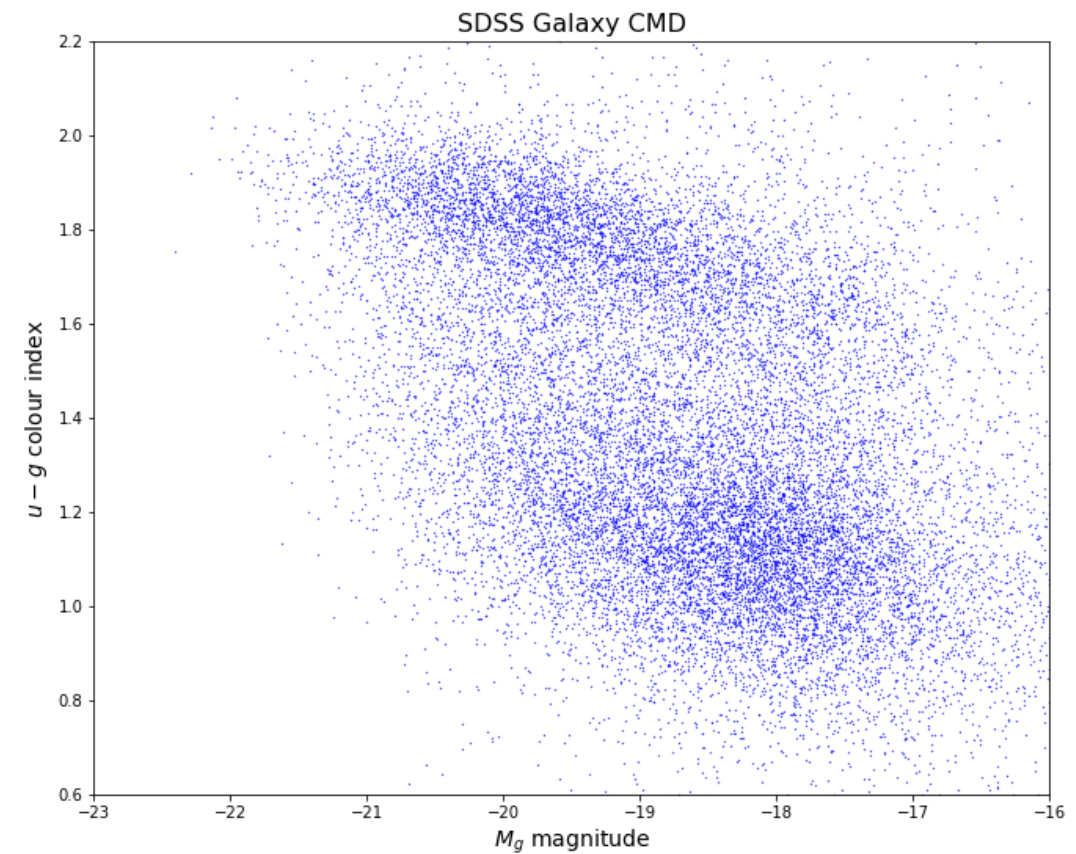
\includegraphics[width=\columnwidth]{images/CMDs/galaxyCMD.PNG}
    \caption{Galaxy colour-magnitude diagram: $u-g$ colour index versus $M_g$ magnitude. The bimodality of the distribution is discussed in the text.}
    \label{fig:CMD1}
\end{figure}